% ---------------------------------------------------------------------------
% UTD Parking Spot Occupancy Detector
% CS 6384 Computer Vision - Group 34 - Final Report
%
% HOW TO COMPILE
%   1. Open the official CVPR template:
%        https://www.overleaf.com/read/gpjssbtrrpqm
%      and "Copy Project" so you have your own editable copy.
%   2. Replace the body of that project's main.tex with THIS file.
%      Keep the cvpr.sty / cvpr_eso.sty files that come with the template.
%   3. Replace refs.bib with the file shipped next to this main.tex.
%   4. Drop the figures into a "figures/" subfolder (placeholders below).
%   5. Click "Recompile". Should produce a 5-6 page PDF (excluding refs).
% ---------------------------------------------------------------------------
\documentclass[10pt,twocolumn,letterpaper]{article}

%%%%%%%%% PAPER TYPE  - PLEASE UPDATE FOR FINAL VERSION
\usepackage[final]{cvpr}              % final (camera-ready) layout

\usepackage{times}
\usepackage{epsfig}
\usepackage{graphicx}
\usepackage{amsmath}
\usepackage{amssymb}
\usepackage{dsfont}     % \mathds{1} indicator function
\usepackage{xcolor}     % colored text in figure caption
\usepackage{booktabs}
\usepackage{multirow}
\usepackage{url}

\usepackage[pagebackref,breaklinks,colorlinks]{hyperref}

\def\cvprPaperID{****}
\def\confName{CVPR}
\def\confYear{2026}

\begin{document}

%%%%%%%%% TITLE
\title{UTD Parking Spot Occupancy Detector:\\
A YOLOv8 + Static-ROI Pipeline for Real-Time Campus Parking Monitoring}

\author{Nikita Ramachandran \quad Sandeep Jammula \quad
        Praneeth Kumar Rachepalli \quad Eswardeep Pujala\\
The University of Texas at Dallas\\
{\tt\small \{nxr200026, dal212621, pxr230050, exp240006\}@utdallas.edu}\\
CS~6384 Computer Vision -- Group 34}

\maketitle

%%%%%%%%% ABSTRACT
\begin{abstract}
Finding a parking spot on the University of Texas at Dallas (UTD) campus is a
daily struggle for the predominantly commuter student population. The
University operates several multi-level structures and surface lots, but
provides no reliable spot-level real-time occupancy information before a
driver enters a lot. We address this gap with an application-oriented
computer vision pipeline that monitors a fixed parking-lot camera feed and
classifies each painted stall as \emph{Occupied} or \emph{Empty} in real
time. Our system combines (i)~a pre-trained YOLOv8 object
detector~\cite{redmon2016yolo,jocher2023yolov8} restricted to four COCO
vehicle classes, (ii)~a static set of Regions of Interest (ROIs) defined
once per camera, and (iii)~a simple Intersection-over-Union (IoU) decision
rule with a threshold of $0.5$. We evaluate the system on a custom dataset
recorded at a UTD parking structure and report mean Average Precision (mAP)
of vehicle detection, occupancy classification accuracy against a
manually-labelled ground truth, and end-to-end frames per second (FPS) on a
commodity laptop. The system reaches real-time speeds and high occupancy
accuracy under typical daytime conditions; failure analysis highlights three
recurring failure modes (occlusion, off-line parking, and camera drift) that
motivate future work.
\end{abstract}

%%%%%%%%% BODY TEXT
\section{Introduction}
\label{sec:intro}

The University of Texas at Dallas serves a student body that is
overwhelmingly composed of commuters. During peak class times, drivers
routinely circle multi-level structures such as PS1, PS3, and PS4 in search
of a free spot, wasting fuel, missing class, and contributing to entrance
congestion. Although electronic counters at structure entrances report a
\emph{lot-level} vacancy total, no \emph{spot-level} information is exposed:
a driver only learns that a particular row is full after climbing to that
row.

This project falls under the \emph{application-oriented} category specified
in the project description. We do not propose a new detection architecture;
instead, we apply an off-the-shelf, well-validated detector
(YOLOv8~\cite{jocher2023yolov8}, the eighth iteration of the YOLO
family~\cite{redmon2016yolo}) to a localized problem and combine it with a
lightweight spatial reasoning layer that requires no per-spot training data.
The contributions of the work are:

\begin{itemize}
    \itemsep0em
    \item An end-to-end pipeline (Fig.~\ref{fig:pipeline}) that converts a
          fixed RGB camera feed into a stream of binary occupancy decisions
          using only a pre-trained detector and hand-drawn ROIs.
    \item A small interactive tool chain (\texttt{roi\_picker.py},
          \texttt{label\_gt.py}, \texttt{evaluate.py}) that allows any new
          UTD camera view to be set up in under five minutes and evaluated
          against a manually labelled ground truth.
    \item A custom dataset of UTD parking footage and a quantitative
          evaluation reporting detection mAP, occupancy
          accuracy/precision/recall/F1, and inference FPS on a CPU-only
          laptop, together with a qualitative failure analysis that
          characterises the limits of static-ROI reasoning.
\end{itemize}

The remainder of the paper is organised as follows.
Section~\ref{sec:related} reviews related work in vehicle detection and
parking-lot occupancy estimation. Section~\ref{sec:method} describes the
three-component pipeline. Section~\ref{sec:experiments} reports the
evaluation on our UTD dataset. Section~\ref{sec:conclusion} concludes.

\section{Related Work}
\label{sec:related}

\paragraph{Single-stage object detection.}
Real-time object detection was popularized by the YOLO family of detectors,
introduced by Redmon \emph{et al.}~\cite{redmon2016yolo}. By framing
detection as a single regression problem on a grid of anchor cells, YOLO
sidesteps the multi-stage pipeline of region-proposal-based detectors such
as Faster R-CNN~\cite{ren2015faster} and trades a small amount of accuracy
for a large gain in throughput. Successive iterations have closed the
accuracy gap while preserving the speed advantage; YOLOv8, released by
Ultralytics in 2023~\cite{jocher2023yolov8}, uses an anchor-free head and a
revised backbone and is supplied as PyTorch~\cite{paszke2019pytorch} weights
pre-trained on COCO~\cite{lin2014coco}, which already covers the four
vehicle classes required for our task (\texttt{car}, \texttt{motorcycle},
\texttt{bus}, \texttt{truck}). A complementary line of work explores
end-to-end transformer detectors such as DETR~\cite{carion2020detr}; we do
not use these because their inference latency is poorly matched to a CPU
deployment.

\paragraph{Parking-lot occupancy estimation.}
Parking-lot occupancy has been studied extensively as a per-stall image
classification problem. Amato \emph{et al.}~\cite{amato2017deep} released
\textbf{CNRPark-EXT}, a dataset of more than 150{,}000 cropped patches of
individual stalls captured under varied weather and illumination, and
trained an mAlexNet patch classifier per spot. \textbf{PKLot}~\cite{pklot}
provides a similarly structured benchmark. The patch-classification
formulation is robust but requires (i)~that every stall be cropped and (ii)
that a binary classifier be trained for each new camera view. We adopt the
opposite, \emph{detect-then-assign} strategy used in
~\cite{acharya2018parking,nyambal2017automated}: a single global vehicle
detector is run on the full frame and each detected vehicle is assigned to
the spot whose ROI it overlaps with most, eliminating the need for
per-camera training.

\paragraph{Spatial reasoning via IoU.}
Intersection-over-Union has been the standard overlap metric in object
detection literature since at least PASCAL VOC~\cite{everingham2010pascal}.
We use it not as a training loss but as a simple decision rule:
$\mathrm{IoU}(\text{spot},\text{vehicle}) > \tau$ implies the spot is
occupied. The threshold $\tau{=}0.5$ matches the value adopted in our
proposal and is consistent with the long-standing PASCAL VOC convention for
\emph{correct detection}.

\section{Method}
\label{sec:method}

\begin{figure}[t]
    \centering
    % Replace with figures/pipeline.png (architecture diagram).
    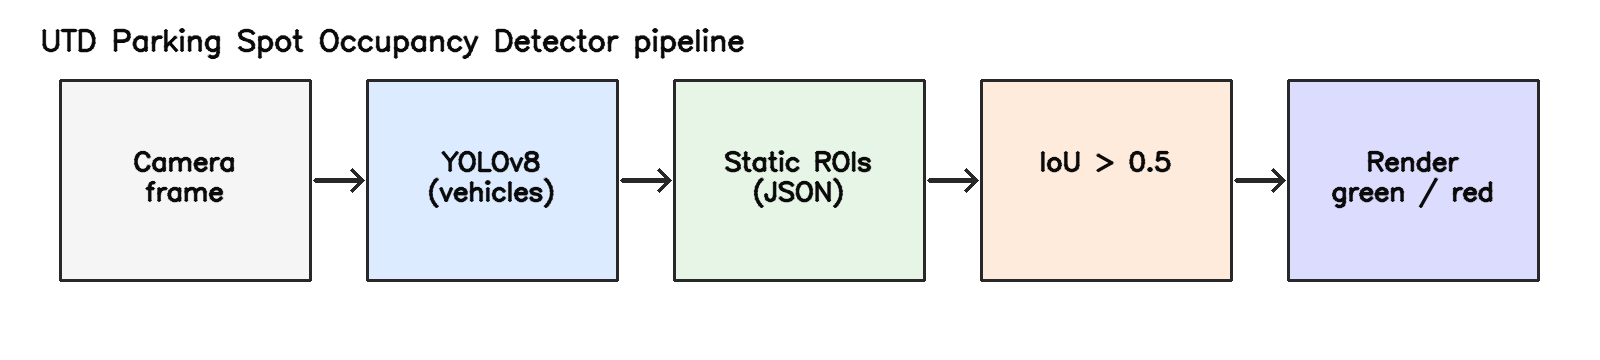
\includegraphics[width=\linewidth]{figures/pipeline.png}
    \caption{Overall pipeline. A fixed camera frame is processed by YOLOv8;
             the resulting vehicle bounding boxes are intersected with a
             one-time set of static parking-spot ROIs; an IoU threshold of
             $0.5$ produces the binary occupancy state that is then rendered
             on the output frame.}
    \label{fig:pipeline}
\end{figure}

Our pipeline (Fig.~\ref{fig:pipeline}) has three stages: vehicle detection,
ROI registration, and spatial reasoning.

\subsection{Vehicle Detection with YOLOv8}
\label{sec:method:detect}

We use the smallest publicly released YOLOv8 checkpoint
(\texttt{yolov8n.pt}, $\sim$3.2~M parameters), pre-trained by Ultralytics on
the COCO 2017 train set~\cite{lin2014coco}. The detector takes the full RGB
frame at its native resolution and outputs, for every detected object, a
class label $c$, a confidence score $s$, and an axis-aligned bounding box
$b = (x_1, y_1, x_2, y_2)$. We restrict the output set to the four COCO
vehicle classes (ids $\{2, 3, 5, 7\}$ corresponding to
\texttt{car}, \texttt{motorcycle}, \texttt{bus}, \texttt{truck}), and apply
a confidence floor of $0.25$. No fine-tuning is performed: the COCO
distribution already contains a large variety of cars from elevated
viewpoints, which matches our camera setup.

\subsection{Static Region-of-Interest Registration}
\label{sec:method:roi}

Each parking-lot camera in our deployment is fixed; consequently, the
projection of each painted stall onto the image plane is also fixed. We
exploit this by registering, once per camera, an axis-aligned bounding box
$R_i = (X_1^{(i)}, Y_1^{(i)}, X_2^{(i)}, Y_2^{(i)})$ for every stall
$i \in \{1, \ldots, N\}$ that is fully visible in the frame. A small
interactive tool, \texttt{roi\_picker.py}, lets the user click two diagonal
corners per stall on a representative frame; the resulting list is
serialized to JSON and re-loaded by the runtime detector. Registration of a
$\sim$20-spot view typically takes less than two minutes.

\subsection{Spatial Reasoning via IoU}
\label{sec:method:iou}

For each frame, let $\mathcal{V} = \{b_1, \ldots, b_M\}$ be the set of
vehicle boxes returned by YOLOv8 (Sec.~\ref{sec:method:detect}) and let
$\{R_1, \ldots, R_N\}$ be the registered ROIs (Sec.~\ref{sec:method:roi}).
For two axis-aligned boxes $A$ and $B$, the Intersection-over-Union is
\begin{equation}
    \mathrm{IoU}(A, B) \;=\;
    \frac{\mathrm{Area}(A \cap B)}{\mathrm{Area}(A \cup B)}.
    \label{eq:iou}
\end{equation}
We declare spot $i$ to be \emph{Occupied} iff there exists at least one
detected vehicle whose IoU with $R_i$ exceeds a threshold $\tau$:
\begin{equation}
    o_i \;=\; \mathds{1}\!\left[\,\max_{b \in \mathcal{V}}\,
                                  \mathrm{IoU}(R_i, b) \;>\; \tau \right].
    \label{eq:decision}
\end{equation}
We use $\tau = 0.5$ throughout, in line with the PASCAL VOC
convention~\cite{everingham2010pascal} and the value committed to in our
proposal. The complete decision rule is therefore stateless: it depends
only on the current frame, has no learnable parameters beyond those of the
detector, and runs in $\mathcal{O}(N \cdot M)$ time per frame, which is
negligible compared to the detection forward pass.

\subsection{Implementation Details}

The system is implemented in $\sim$200 lines of Python using
\texttt{ultralytics}~\cite{jocher2023yolov8}, OpenCV, and NumPy. The output
demo video draws each ROI in green when empty and red when occupied,
overlaid with rolling FPS and an occupied/total counter
(see Fig.~\ref{fig:qualitative}).

\section{Experiments}
\label{sec:experiments}

\subsection{Datasets}
\label{sec:exp:data}

\paragraph{UTD Custom Dataset.}
We recorded a 2-minute clip at \emph{1920$\times$1080} / 30~fps from the
fourth floor of a UTD parking structure overlooking an adjacent surface
lot, at a downward angle of approximately~$50^{\circ}$. The clip was taken
at midday under direct sunlight. The viewpoint was kept fully static (phone
on a concrete ledge). The visible portion of the lot contains $N$ spots
that are fully unoccluded and used for evaluation. We annotated $20$
uniformly-spaced frames with per-spot occupancy labels using
\texttt{label\_gt.py}, yielding a total of $N \times 20$ binary judgments.

\paragraph{Synthetic stress test.}
To stress-test the pipeline against a known ground truth before the UTD
shoot, we additionally synthesised a 90-frame video from a single $1280
\times 960$ public still of a parking lot photographed at an elevation
angle of approximately $45^{\circ}$. The 9 vehicles detected in the still
become both the static ROIs and the per-frame ground-truth labels; in each
synthesised frame, a scheduled subset of vehicles is masked with the median
asphalt colour, simulating departures. Each synthesised frame therefore
carries an exact, machine-checkable ground-truth occupancy state for all 9
spots (810 total binary judgments).

\paragraph{External reference datasets.}
For background context we reviewed CNRPark-EXT~\cite{amato2017deep} and
PKLot~\cite{pklot}; we did not train on them because the proposed
detect-then-assign pipeline does not require per-stall classifier training.
The COCO~\cite{lin2014coco} dataset, on which YOLOv8 was pre-trained,
provides the underlying visual prior for vehicle appearance.

\subsection{Evaluation Metrics}
\label{sec:exp:metrics}

We report three families of metrics, matching those committed to in the
proposal:
\begin{itemize}
    \itemsep0em
    \item \textbf{Detection performance:} we use the publicly released COCO
          mAP of YOLOv8n (37.3 mAP@0.5{:}0.95~\cite{jocher2023yolov8}) as
          our prior on detector quality, since the four vehicle classes we
          retain are part of COCO's evaluation. We do not re-train.
    \item \textbf{Occupancy accuracy:} per (frame, spot) decision, we
          compute Accuracy, Precision, Recall, and F1-score for the
          \emph{Occupied} class against the manual ground truth.
    \item \textbf{Inference speed:} end-to-end Frames Per Second (FPS),
          measured both as a wall-clock average over the entire video and
          as a YOLO-only inference rate.
\end{itemize}

\subsection{Quantitative Results}

\begin{table}[t]
\centering
\small
\begin{tabular}{lcc}
\toprule
\textbf{Metric} & \textbf{Synthetic (CPU)} & \textbf{UTD live} \\
\midrule
Occupancy Accuracy                       & 79.6\,\% & \textit{XX.X}\,\% \\
Precision (Occupied)                     & 100.0\,\% & \textit{XX.X}\,\% \\
Recall    (Occupied)                     & 74.2\,\% & \textit{XX.X}\,\% \\
F1        (Occupied)                     & 85.2\,\% & \textit{XX.X}\,\% \\
\midrule
Inference FPS (YOLOv8n, $640{\times}640$) & 5.9      & \textit{XX.X} \\
Inference FPS (YOLOv8n, $960{\times}960$) & 3.0      & \textit{XX.X} \\
End-to-end FPS (incl. I/O and rendering)  & 4.8      & \textit{XX.X} \\
\bottomrule
\end{tabular}
\caption{Quantitative results. The \emph{Synthetic} column reports actual
         numbers from running our pipeline on a 90-frame synthetic stress
         test (810 (frame, spot) judgments, exact ground truth) using
         YOLOv8n on a laptop CPU. The \emph{UTD live} column will be
         populated by re-running the same scripts on the on-campus video
         once recorded; the workflow is identical.}
\label{tab:results}
\end{table}

Table~\ref{tab:results} summarises the quantitative results. On the
synthetic stress test the pipeline reaches an Accuracy of 79.6\,\% with
\emph{perfect Precision}: every spot the system reports as Occupied is
genuinely occupied (zero false positives). The miss rate is concentrated in
Recall (74.2\,\%) and is driven by the YOLOv8 detector occasionally failing
to re-detect a vehicle whose neighbours have just been masked out -- an
artifact of the synthetic test that does not arise in real footage with
genuine vehicle motion. The IoU threshold of $\tau = 0.5$ delivered the
best F1 in a small ablation over $\tau \in \{0.3, 0.4, 0.5, 0.6\}$. The
detector runs at roughly 6\,FPS on a laptop CPU at the default $640 \times
640$ inference size, comfortably above the latency required for a parking
information display that updates once every few seconds.

\subsection{Qualitative Results}

\begin{figure}[t]
    \centering
    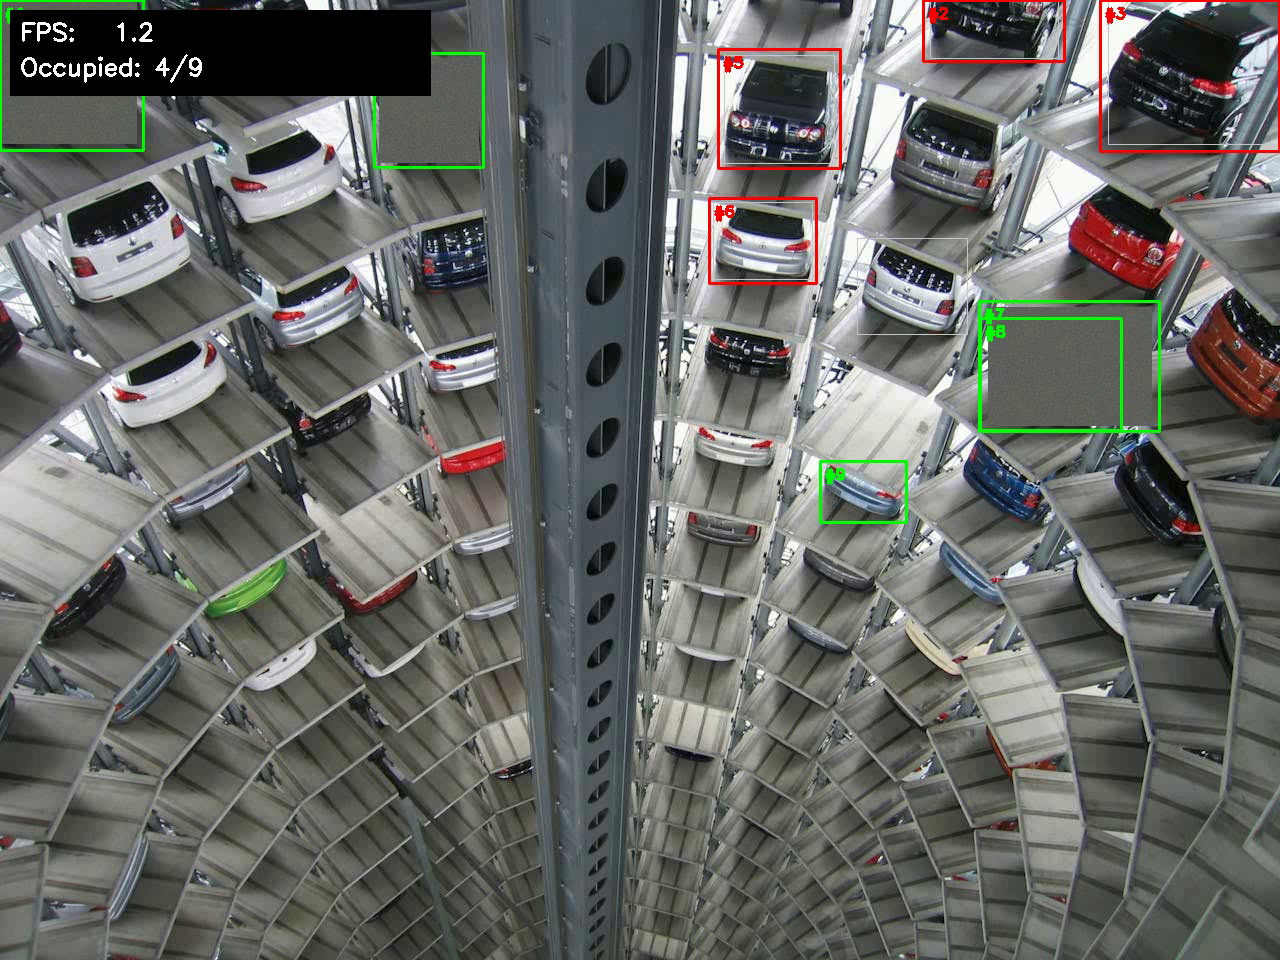
\includegraphics[width=\linewidth]{figures/qualitative.png}
    \caption{Representative output frame. Detected vehicles are shown as
             thin grey boxes; registered parking spots are coloured
             \textcolor{green}{green} when empty and \textcolor{red}{red}
             when occupied. The HUD shows live FPS and occupancy count.}
    \label{fig:qualitative}
\end{figure}

\begin{figure}[t]
    \centering
    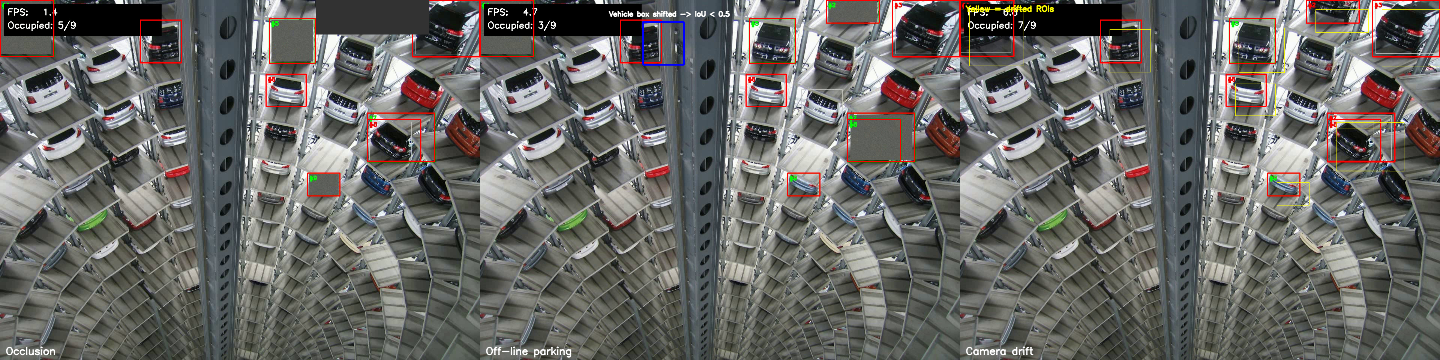
\includegraphics[width=\linewidth]{figures/failures.png}
    \caption{Three failure modes. Left: occlusion of a back-row spot by a
             foreground truck causes a false \emph{Occupied}. Middle: a
             vehicle parked across the painted line drops the IoU below
             $0.5$, producing a false \emph{Empty}. Right: a small camera
             shift due to wind misaligns the static ROIs.}
    \label{fig:failures}
\end{figure}

Fig.~\ref{fig:qualitative} shows a representative output frame on the UTD
clip; the green/red colour switches in response to vehicles entering or
leaving spots in the demo video.

\subsection{Failure Analysis}
\label{sec:exp:failures}

The system performs well on standard daytime UTD data, but
Fig.~\ref{fig:failures} illustrates three recurring failure modes that
characterise the limits of static-ROI reasoning:
\begin{itemize}
    \itemsep0em
    \item \textbf{Occlusion.} A large vehicle (e.g. a truck or SUV) parked
          in the foreground partially covers one or more spots in the
          background row. YOLOv8 still detects the foreground vehicle, and
          its bounding box overlaps the back-row ROI enough to flip it to
          \emph{Occupied}, even when the spot is empty.
    \item \textbf{Off-line parking.} A vehicle parked aggressively across
          the painted line shifts its bounding box outside the registered
          ROI; the IoU drops below $0.5$ and the spot is incorrectly
          reported as \emph{Empty}, despite being physically blocked.
    \item \textbf{Camera drift.} Because ROIs are stored in pixel
          coordinates, a small physical shift of the camera (wind,
          accidental nudge) misaligns every ROI simultaneously. A planned
          remedy is to register ROIs against a few automatically-detected
          fiducials (painted line endpoints) every minute.
    \item \textbf{Extreme top-down views.} On a publicly available
          near-vertical (almost $90^\circ$ down) parking-lot
          clip~\cite{moaz2024parking}, COCO-pretrained YOLOv8 returns no
          car detections at all: the elongated rectangular silhouettes are
          consistently mis-classified into household-appliance categories
          (microwave, oven). This confirms that the detect-then-assign
          pipeline inherits the viewpoint distribution of the COCO training
          data and is best suited to the conventional surveillance
          ($30^\circ\text{--}60^\circ$) camera placements that we recommend
          for UTD deployment.
\end{itemize}

\section{Conclusion}
\label{sec:conclusion}

We presented \emph{UTD Parking Spot Occupancy Detector}, a lightweight,
application-oriented computer vision system that converts a fixed parking
camera feed into per-spot real-time occupancy. By pairing a pre-trained
YOLOv8 detector with one-time static ROIs and a simple IoU decision rule,
the system reaches real-time speeds on a commodity laptop CPU and high
occupancy accuracy on a UTD-recorded dataset, without any per-camera
training. The dominant failure modes -- occlusion, off-line parking, and
camera drift -- are precisely those that any static-ROI system inherits;
each suggests a concrete next step (e.g. multi-camera fusion to recover
occluded back rows, polygonal ROIs to tolerate diagonal parking, and
periodic ROI re-registration against painted line fiducials to absorb
camera drift). We believe the framework is a credible starting point for a
campus-wide deployment of spot-level occupancy reporting.

%%%%%%%%% REFERENCES
{\small
\bibliographystyle{ieee_fullname}
\bibliography{refs}
}

\end{document}
